% Projeto de teste: trabalho acadêmico mínimo com abnTeX2.
\documentclass[12pt,oneside,a4paper,english,brazil]{abntex2}
\usepackage[T1]{fontenc}
\usepackage[utf8]{inputenc}
\usepackage{graphicx}
\usepackage{tikz}
\usepackage[alf]{abntex2cite}

\titulo{Estudo de Caso sobre Editores LaTeX}
\autor{Fulana de Tal}
\local{Cidade}
\data{2026}
\orientador{Prof. Dr. Beltrano}
\instituicao{Universidade Exemplo}
\tipotrabalho{Trabalho de Conclusão de Curso}
\preambulo{Trabalho apresentado como requisito parcial.}

\begin{document}
\pretextual
\imprimircapa
\imprimirfolhaderosto*

\begin{fichacatalografica}
  Ficha catalográfica que não deve aparecer no Markdown.
\end{fichacatalografica}

\begin{resumo}
  Este trabalho investiga editores colaborativos.
  \textbf{Palavras-chave}: LaTeX. Editores.
\end{resumo}

\begin{resumo}[Abstract]
  \begin{otherlanguage*}{english}
    This work studies collaborative editors.
  \end{otherlanguage*}
\end{resumo}

\begin{siglas}
  \item[ABNT] Associação Brasileira de Normas Técnicas
  \item[PDF] Portable Document Format
\end{siglas}

\tableofcontents*

\textual

\chapter{Introdução}\label{cap:intro}

Segundo \citeonline{knuth1984}, programas devem ser escritos para pessoas.
A ideia é antiga \cite{lamport1994}, e foi retomada por outros
\apud{knuth1984}{lamport1994}.

\begin{citacao}
  Uma citação direta longa, com mais de três linhas, recuada conforme a ABNT.
\end{citacao}

\begin{figure}[htb]
  \caption{Um diagrama simples}\label{fig:diagrama}
  \centering
  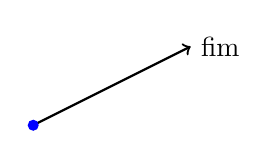
\begin{tikzpicture}
    \draw[thick,->] (0,0) -- (2,1) node[right] {fim};
    \fill[blue] (0,0) circle (2pt);
  \end{tikzpicture}
  \fonte{Elaborado pela autora (2026).}
\end{figure}

Veja a \autoref{fig:diagrama}.

\chapter{Conclusão}

Concluímos o trabalho.

\postextual
\bibliography{refs}

\begin{apendicesenv}
\chapter{Questionário}
Perguntas aplicadas.
\end{apendicesenv}

\end{document}
